\chapter{Linux}

\section{Navegación entre Directorios}
Uno de los usos principales del shell de bash es la navegación entre directorios (carpetas). Los principales comandos para esta sección son:

\begin{lstlisting}
    # Check the current directory path
    pwd

    # List files and directories
    ls

    # Change to the specified directory
    cd /path/to/directory        

    # More information about the ls command
    ls --help
\end{lstlisting}

\subsection*{Ejemplo}
\begin{figure}[h!]
    \centering
    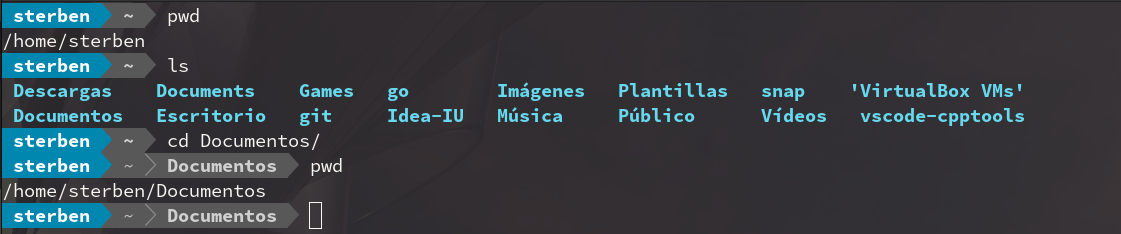
\includegraphics[width=1\textwidth]{img/navegacion.png}
\end{figure}

\newpage

\subsection{Visualización}
Existen paquetes como \textbf{tree} que permiten ver la estructura de directorios en formato de árbol.

\begin{lstlisting}
    # Install the tree package
    sudo apt install tree

    # Use the tree command to display the directory structure
    tree /path/to/directory      
\end{lstlisting}

\textbf{Nota:} El comando `apt` es un gestor de paquetes utilizado en algunas distribuciones de Linux. Dependiendo del sistema operativo que estés usando, encontrarás diferentes gestores de paquetes. El siguiente ejemplo se presenta para \textbf{Fedora 40}, que utiliza el gestor de paquetes `dnf`.

Puedes encontrar más información sobre los diferentes gestores de paquetes en Linux en este 
\href{https://www.profesionalreview.com/2016/09/11/gestor-de-paquetes-en-linux/#:~:text=DNF%20es%20el%20gestor%20de,en%20CentOS%20en%20el%20futuro.&text=Probando%20los%20diferentes%20gestores%20de,que%20te%20resulte%20m%C3%A1s%20c%C3%B3modo.}{\textcolor{blue}{enlace}}:

\subsection*{Ejemplo}
\begin{figure}[h!]
    \centering
    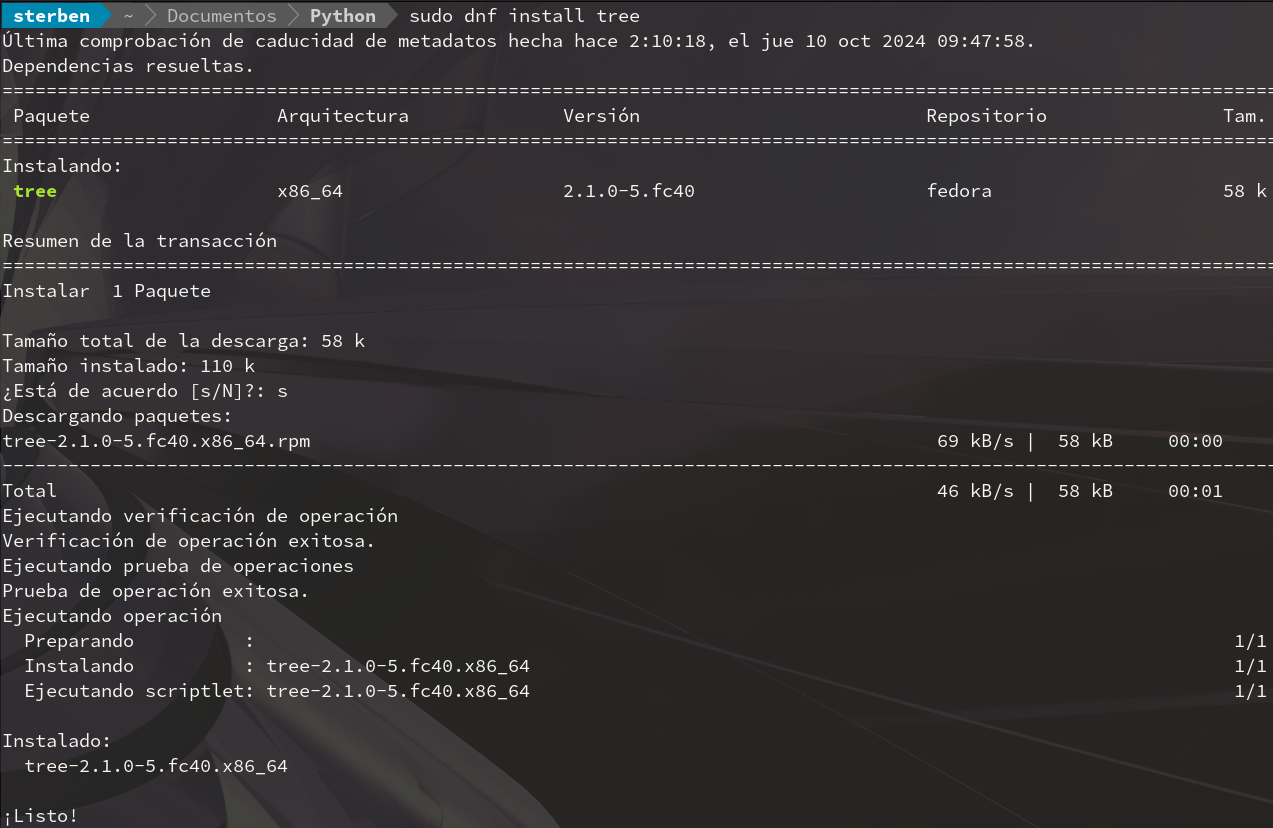
\includegraphics[width=0.8\textwidth]{img/visuali1.png}
    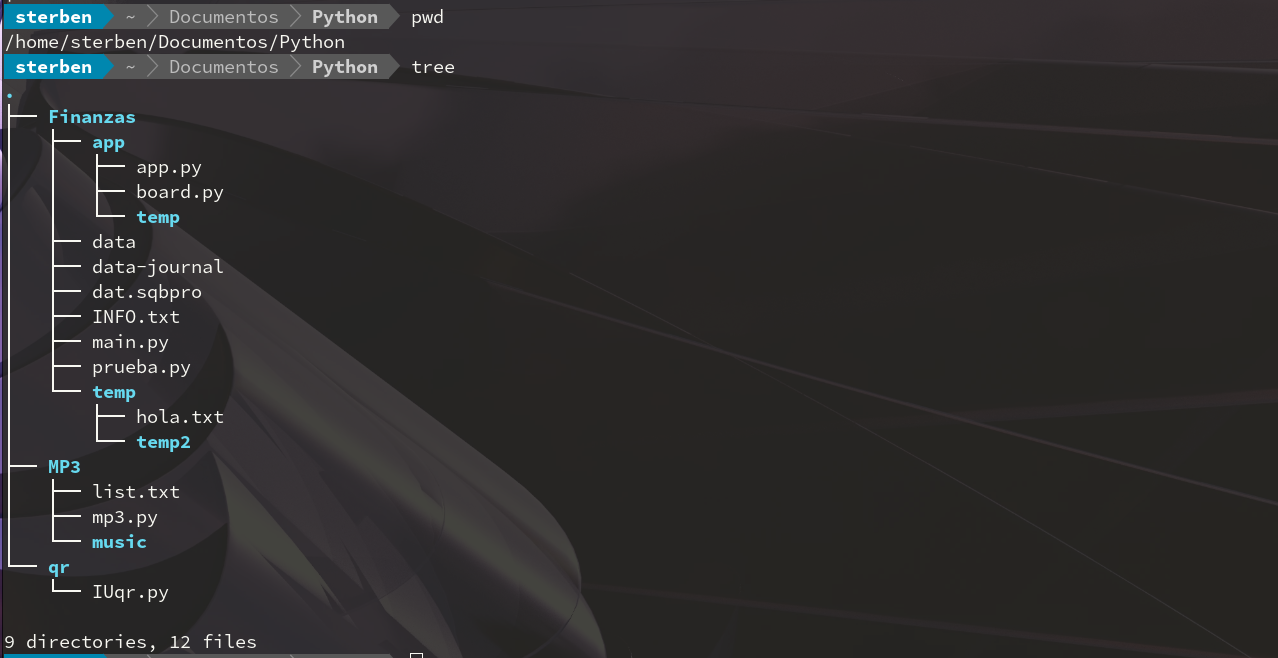
\includegraphics[width=0.8\textwidth]{img/visuali2.png}
\end{figure}

\subsection{Permisos}
En el ejemplo anterior, al instalar un paquete, se solicita la contraseña. Esto ocurre porque necesitamos permisos de \textbf{superusuario} (superUser). Además, es posible verificar los permisos de cada directorio y archivo desde la consola.

En Linux, los permisos se representan con las siguientes letras:
\begin{itemize}
    \item \textbf{d}: indica un directorio.
    \item \textbf{r}: permite la lectura.
    \item \textbf{w}: permite la escritura.
    \item \textbf{x}: permite la ejecución.
\end{itemize}

Para verificar los permisos, utilizaremos un comando que ya aprendimos, que es \textbf{ls}. Al verificar más datos con \textbf{ls --help}, podemos observar que hay opciones que nos permiten listar todos los directorios y archivos con sus respectivos permisos:

\begin{lstlisting}
    # List files and directories
    ls

    # List files and directories with detailed information 
    ls -l     

    # List all files and directories, including hidden ones, with detailed information
    ls -la
\end{lstlisting}

\subsection*{Ejemplo}
\begin{figure}[h!]
    \centering
    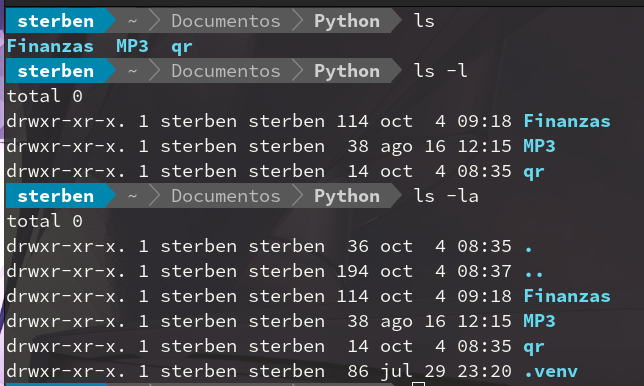
\includegraphics[width=0.9\textwidth]{img/permisos.png}
\end{figure}

\subsubsection*{Explicación}
\begin{lstlisting}
    drwxr-xr-x. 1 sterben1 sterben2 114 oct  4 09:18 Finanzas
\end{lstlisting}

\begin{itemize}
    \item \textbf{d}: directorio.
    \item \textbf{rwx}: el propietario \textbf{sterben1} tiene permisos de lectura, escritura y ejecución.
    \item \textbf{r-x}: el grupo \textbf{sterben2} tiene permisos de lectura y ejecución.
    \item \textbf{r-x}: otros (también \textbf{sterben2}) tienen permisos de lectura y ejecución.
    \item \textbf{114}: tamaño en bytes (no representa el valor real).
    \item \textbf{oct 4 09:18}: fecha de la última modificación.
    \item \textbf{Finanzas}: nombre del directorio.
\end{itemize}

\section{Gestor de Archivos y Directorios}
En este apartado, veremos operaciones básicas como copiar, mover, eliminar o crear diferentes archivos y directorios.

\begin{lstlisting}
    # Copy a file to a specific destination
    cp archivo destino

    # Move a file to a new destination, renaming it if necessary
    mv archivo destino     

    # Remove a file
    rm archivo

    # Create a new directory
    mkdir nombreDirectorio

    # Remove an empty directory
    rmdir nombreDirectorio
\end{lstlisting}
